\documentclass[tikz]{standalone}


\usepackage{tikz}
\usetikzlibrary{calc}

\begin{document}
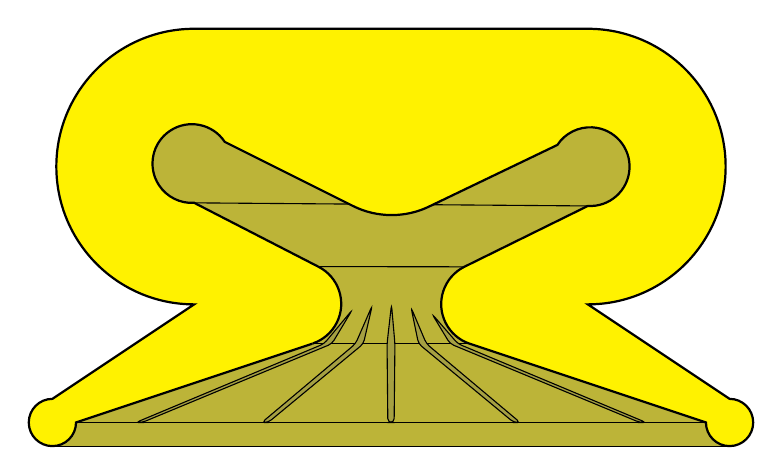
\begin{tikzpicture}

%\foreach \x in {-5,-4, ...,5}{
%	\draw[help lines] (\x,-5)node[below]{\x} -- (\x,5);
%}
%\foreach \y in {-5,-4, ...,5}{
%	\draw[help lines] (-5,\y)node[left]{\y} -- (5,\y);
%}


\pgfmathsetmacro{\alp}{atan(1/3)}
\pgfmathsetmacro{\bet}{atan(1/2)}


\path
(-1, 1)coordinate(1L)--(-4,0)coordinate(2L)arc(0:-270:.3)--(-2.5,1.5)arc(-90:-270:1.75)--(2.5,5)arc(90:-90:1.75)--(4.3,.3)arc(90:-180:.3)coordinate(2R)--(1,1)coordinate(1R)
arc(-90-\alp:-270+\bet:.53)coordinate(3R) --(2.5,2.75)coordinate(4R)arc(\bet-90-30:\bet+90+30:.5) -- (.5,2.75)arc(-90+\bet:-90-\bet:1.1)--++(180-\bet:1.82)arc(90-\bet-30:270-\bet+30:.5)coordinate(4L)--(-.925,1.98)coordinate(3L)arc(90-\bet:-90+\alp:.53) %--cycle
;

\fill[yellow!70!black]
(2R)--(1,1)coordinate(1R)
arc(-90-\alp:-270+\bet:.53)coordinate(3R) --(2.5,2.75)coordinate(4R)arc(\bet-90-30:\bet+90+30:.5) -- (.5,2.75)arc(-90+\bet:-90-\bet:1.1)--++(180-\bet:1.82)arc(90-\bet-30:270-\bet+30:.5)coordinate(4L)--(-.925,1.98)coordinate(3L)arc(90-\bet:-90+\alp:.53)--(-4,0)--++(-.3,-.3)--($(2R)+(.3,-.3)$)
;

\draw (1L) -- (1R);
\draw (2L) -- (2R);
\draw (3L) -- (3R);
\draw (4L) -- (4R);
\draw (2L)++(-.3,-.3)--($(2R)+(.3,-.3)$);


\foreach \pos in {.1,.3, .5, .7, .9}{
	\path (1L)--(1R)coordinate[pos=\pos-.025](11);
	\path (1L)--(1R)coordinate[pos=\pos+.025](12);
	\path (2L)--(2R)coordinate[pos=\pos-.005](21);
	\path (2L)--(2R)coordinate[pos=\pos+.005](22);

	\draw[fill=yellow!60!black,
	rounded corners = .5mm	
	] (11)--(21)--(22)--(12)--++(50+90*\pos:.5)--cycle; %  node{2};
}


\draw[
	thick,
	fill=yellow,
%	rounded corners=1mm
] 
(-1, 1)coordinate(1L)--(-4,0)coordinate(2L)arc(0:-270:.3)--(-2.5,1.5)arc(-90:-270:1.75)--(2.5,5)arc(90:-90:1.75)--(4.3,.3)arc(90:-180:.3)coordinate(2R)--(1,1)coordinate(1R)
arc(-90-\alp:-270+\bet:.53)coordinate(3R) --(2.5,2.75)coordinate(4R)arc(\bet-90-30:\bet+90+30:.5) -- (.5,2.75)arc(-90+\bet:-90-\bet:1.1)--++(180-\bet:1.82)arc(90-\bet-30:270-\bet+30:.5)coordinate(4L)--(-.925,1.98)coordinate(3L)arc(90-\bet:-90+\alp:.53) %--cycle
;


\end{tikzpicture}
\end{document}